%!TEX root = ../main.tex






\iffalse
\section{Problem Discussion}

\subsection{Ours}

In Section~\ref{sec:pre}, we have an important mapping $\phi$, \ie $\phi(i) = j, i\in[1,|T|],  j\in[1,|C|]$. $\phi(i) = j$ denotes that we will assign  $t_i$ to $c_j$ and use $\df_{\gamma(j)}$  to represent $\df_i$. Each $t_i$ will be assigned to one and only one $c_j$, but each  $c_j$ might be assigned with multiple tuples in $\train$. 

Consider Eq.~\ref{eqa:expectation}, an important question is how to efficiently compute $\mathrm{E}[\sum_{i\in \train} \min_{j\in \core} d_{ij}]$. Suppose that we first enumerate all possible worlds, then all tuples are deterministic. Thus, we can easily compute
\begin{equation}
	\label{eq:possible_worlds}
	\begin{aligned}
		\mathrm{E}[\sum_{i\in \train} \min_{j\in \core} d_{ij}] & = \sum_{k = 1}^{P} p_{k} * sum_k \\
		& = \sum_{k = 1}^{P} p_{k} * (\sum_{i=1}^{|T|}d_{i, \phi(i)}) \\
		& = \sum_{i=1}^{|T|} \sum_{k = 1}^{P} p_{k} * d_{i, \phi(i)} \\
	\end{aligned}
\end{equation}
where $P$ is the number of possible worlds, $p_{k}$ denotes the probability of occurrence of the $k$-th possible world. Naturally, we have $\sum_{k = 1}^{P} p_{k} = 1$.

Then,  we can aggregate same $d_{i, \phi(i)}$. Suppose we have $d_{g_1}, \cdots, d_{g_C}$. 
\begin{equation}
	\begin{aligned}
		\mathrm{E}[\sum_{i\in \train} \min_{j\in \core} d_{ij}] 
		 = \sum_{i=1}^{|T|} ( &
		 d_{g_1} * (p_{m_1}+\cdots+p_{{m_2} - 1})  \\
		+ & d_{g_2}* (p_{m_2}+\cdots+p_{{m_3} - 1}) \\
		+ & \cdots \\
		+ &  d_{g_C}* (p_{m_C}+\cdots+p_{P}) )
	\end{aligned}
\end{equation}


In practice, we have a reasonable assumption that the imputation of each tuple is independent. For tuple $t_i$, $t_i$ has $\Psi(i)$ imputation schemes and the probability of each scheme is $\rho$.

Every time we compute the utility of a new tuple, we suppose that each tuple in the coreset is already imputed. Then, we have
\begin{equation}
	\begin{aligned}
	\mathrm{E}[\sum_{i\in \train} \min_{j\in \core} d_{ij}] = \sum_{i=1}^{|T|} \sum_{k=1}^{\Psi(i)} \rho_{k} * d_{i, \phi(i)} 
	\end{aligned}
\end{equation}

 
For a new tuple $c$, we suppose that tuple $c$ has a missing value. Consider that $c$ has $\Pi$ different values, \ie $c^{(1)}, \cdots, c^{(\Pi)}$. The probability of each value $c^{(l)}$ is $\pi_{l}$. $\phi_{l}(i)=j$ indicates that when  $c = c^{(l)}$, we assign  $t_i$ to $c_j$.

\begin{equation}
	\mathrm{E}[\sum_{i\in \train} \min_{j\in \core} d_{ij}]  = \sum_{i=1}^{|T|} \sum_{k=1}^{\Psi(i)} \rho_{k} * (\sum_{l=1}^{\Pi} \pi_{l} * d_{i, \phi_{l}(i)}) 
\end{equation}

\subsection{Miao's}

Miao's derivation is similar to ours. 

We assume that for each tuple $x_i$ in $T$, $x_i$ has a corresponding set of tuples $A_i$. Specifically, if there is no missing value in $x_i$, then $x_i$  has been assigned. If there are missing values in $x_i$, then we need to choose a tuple from $A_i$ to replace $x_i$. Similar for tuples in $\core$, each one has a corresponding set $B_i$. Without loss of generality, we can assume that the size of each $A_i$ and $B_i$ is $L$.

Then, we can define a assignment $\varphi: \{x_1, \cdots, x_{|T|}, y_1, \cdots, y_{|\core|}\} \rightarrow \A_1 \times \cdots \times A_{|T|} \times B_1 \times \cdots \times B_{|\core|}$. Then, given an assignment $\varphi$, we can compute the distance between $x_i$ and $y_j$ 
\begin{equation}
	d_{ij}(\varphi) = d[\varphi(x_i), \varphi(y_j)]
\end{equation}
We use $c_i(\varphi) = \min_j d_{ij}(\varphi)$ to denote the minimum distance between $x_i$ and the tuple in $\core$ given the assignment $\varphi$. For each assignment $\varphi$, our goal is to compute $s(\varphi) = c_1(\varphi) + \cdots + c_{|T|}(\varphi)$. 

Apparently, each assignment $\varphi_i$ has a probability $p_i$. Thus, we can rewrite Eq.~\ref{eq:possible_worlds} as 
\begin{equation}
		\begin{aligned}
		\mathrm{E}[\sum_{i\in \train} \min_{j\in \core} d_{ij}] & = \sum_{k = 1}^{P} p_{k} * sum_k \\
		& = \sum_{k = 1}^{P} p_{k} * s(\varphi_k) \\
		& = \sum_{k = 1}^{P} p_{k} * \sum_{i=1}^{|T|} c_i(\varphi_k) \\
		& = S \\
	\end{aligned}
\end{equation}


\begin{figure*}[t]
	\centering
	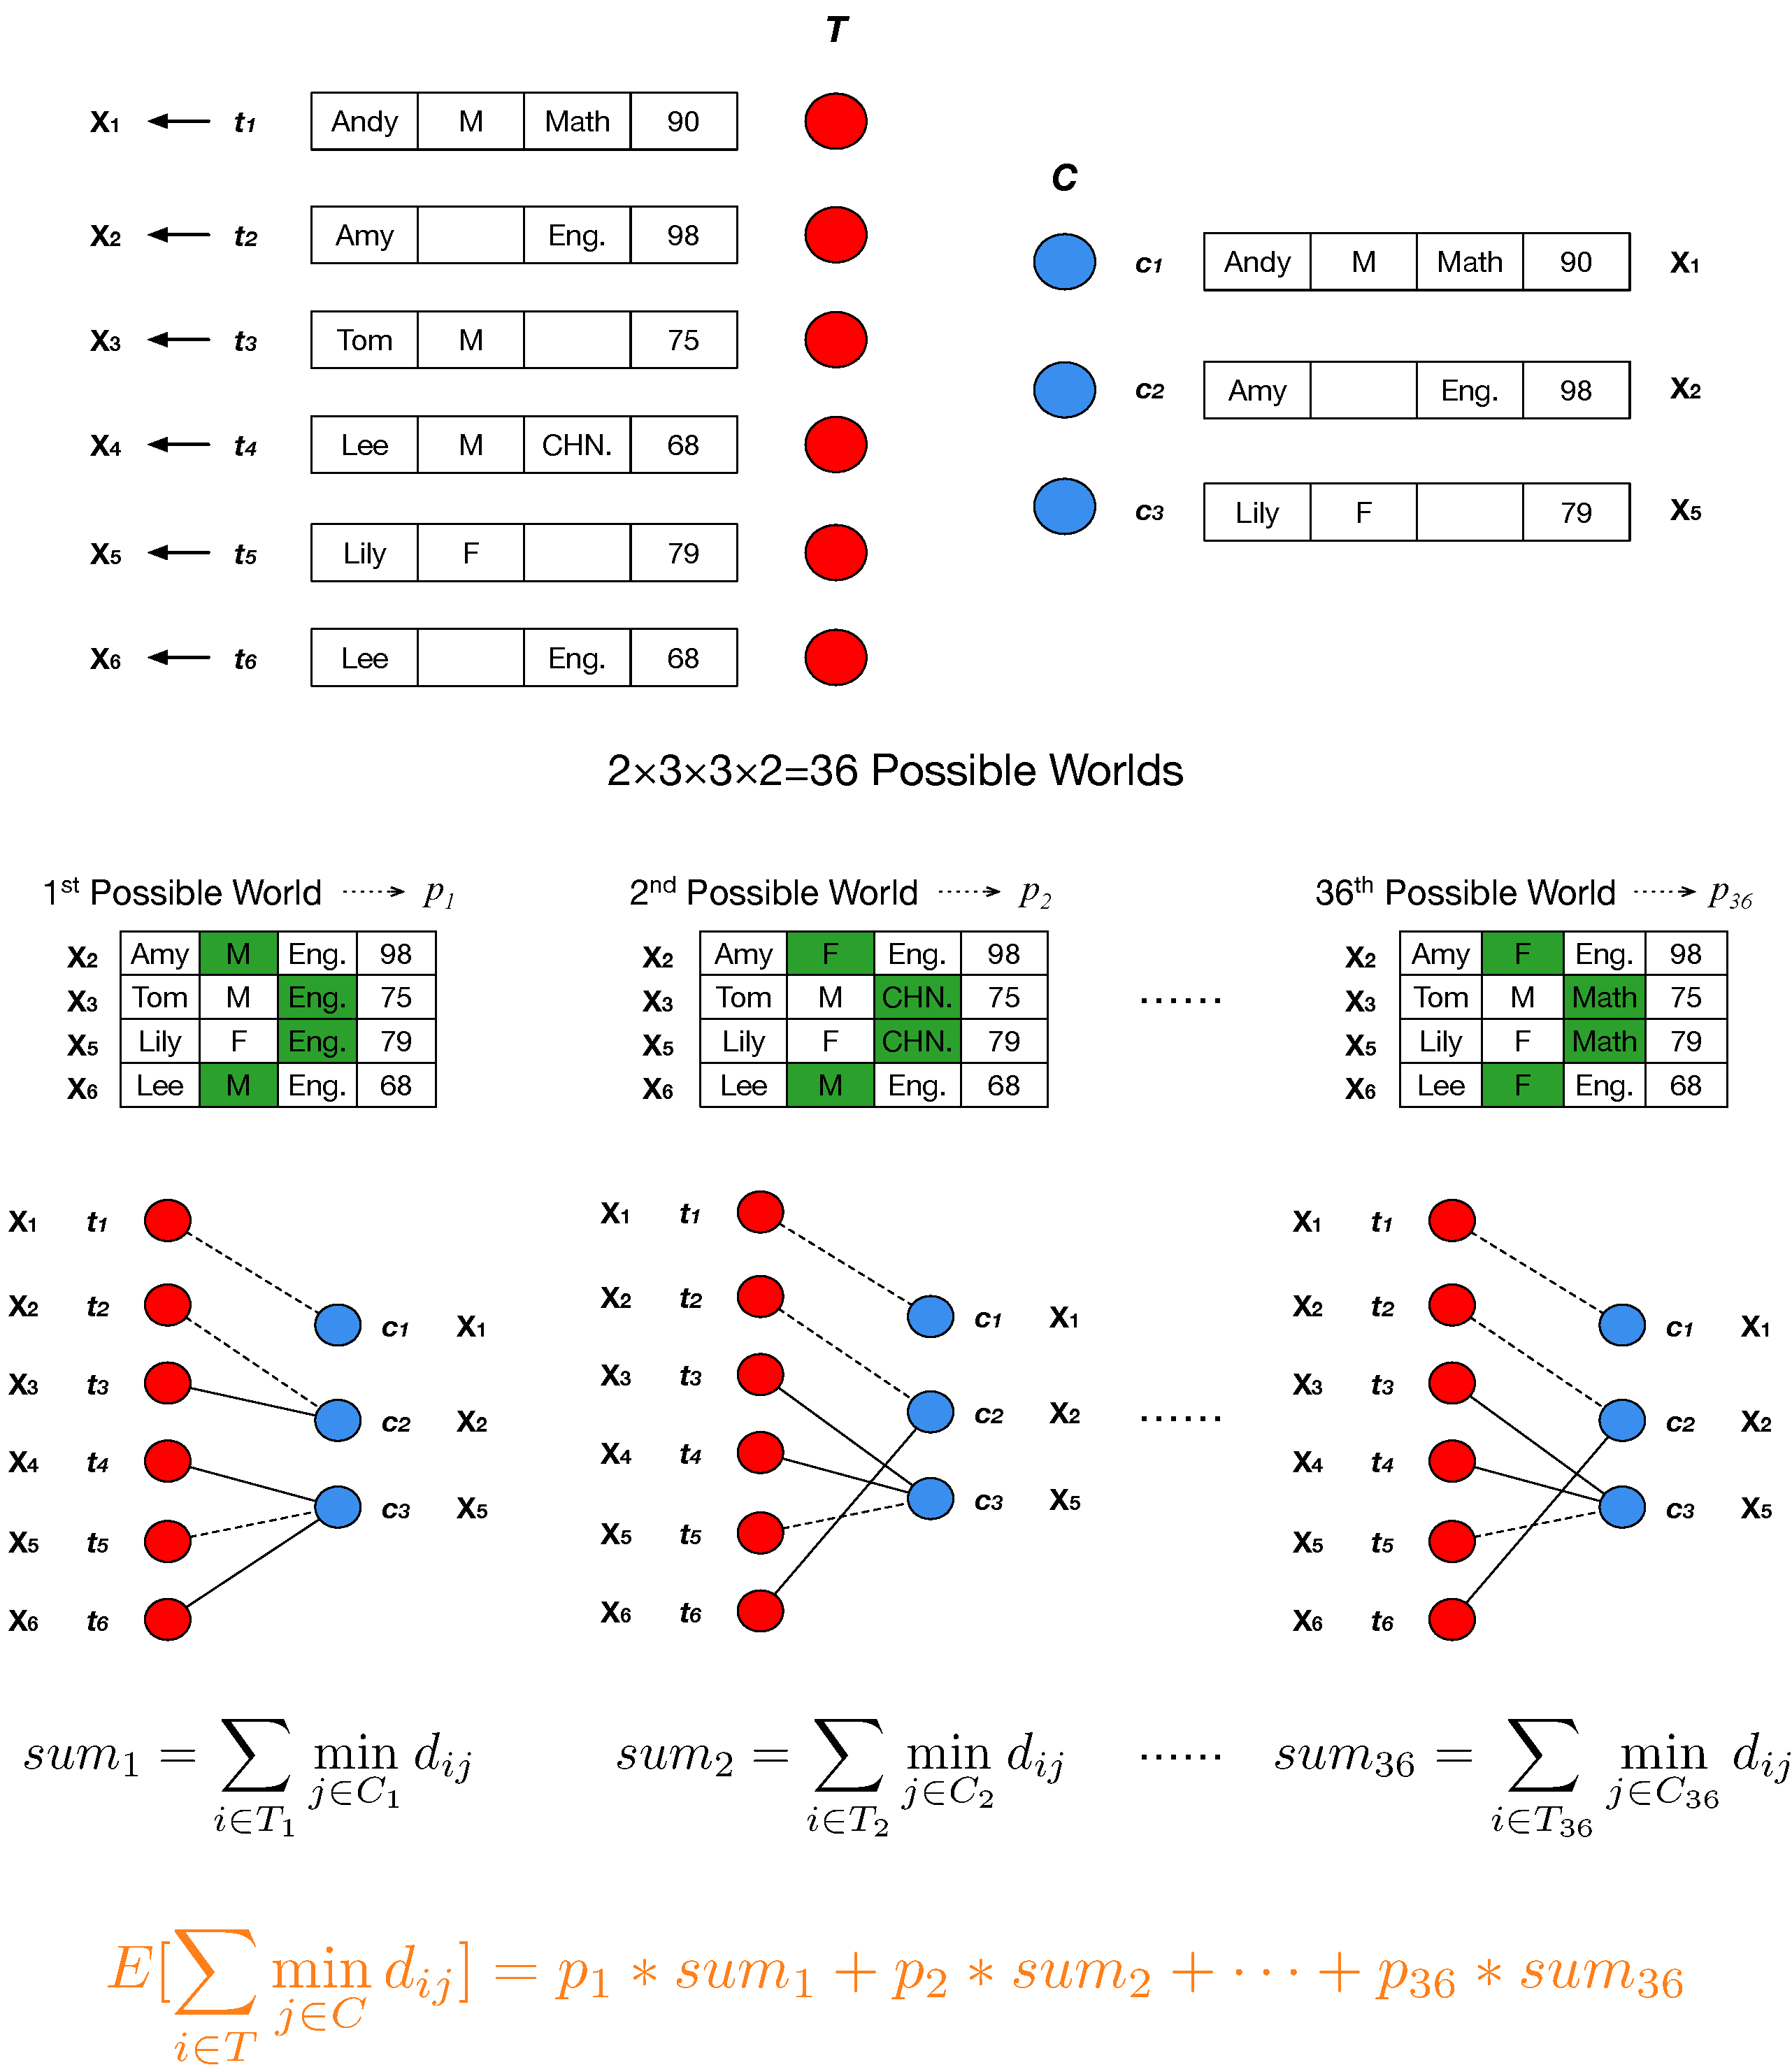
\includegraphics[width=0.98\textwidth]{figs/example.pdf}
	\caption{An example of Coreset4DC.}
	\label{fig:frog}
\end{figure*}
\fi


